\subsection{Hello World}
\subsubsection{Introduction}

One of the most simple way of programming Sunway TaihuLight is to use only the
MPE
(Management Processing Element).
The MPE can be programmed in vanilla C/C++. Let us first write some program
that run on MPE.




\subsubsection{Source code}
 We have compiled and executed the following source codes:

\verb`master.c`
\begin{code}
#include <stdio.h>
#include <athread.h>
#include <fcntl.h>
#define N 4096


//extern SLAVE_FUN(func)();

double a[N];
double b[N];
double c[N];

int main() {
  int i;
  printf("hello Sunway TaihuLight\n");

  for (i=0; i<N;++i){
    a[i] = i;
    b[i] = i;
  }

  for (i=0; i<N;++i){
    c[i] = a[i] * b[i];
  }

  for (i=1; i<N; i=2*i+1){
    printf("%d^2 == %lf\n", i, c[i]);
  }

  return 0;
}

\end{code}

\verb`run.sh`
\begin{code}

cd /home/export/base/nsccwuxi_riken/riken/online1/sandbox/nushio_box/sunway-test/01-master/src/
make && make run
    
\end{code}

\subsubsection{Results}

Got the following results:

\begin{code}
# 2017-02-15 00:20:49.556760
$ chmod 755 /home/nushio/hub/GB17/sunway-test/01-master/src/run.sh
$ ssh sunway 'mkdir -p /home/export/base/nsccwuxi_riken/riken/online1/sandbox/nushio_box/sunway-test/01-master/src/'
$ rsync -avz /home/nushio/hub/GB17/sunway-test/01-master/src/ sunway:/home/export/base/nsccwuxi_riken/riken/online1/sandbox/nushio_box/sunway-test/01-master/src/
sending incremental file list
./
Makefile
run.sh

sent 436 bytes  received 72 bytes  145.14 bytes/sec
total size is 955  speedup is 1.88
$ ssh sunway /home/export/base/nsccwuxi_riken/riken/online1/sandbox/nushio_box/sunway-test/01-master/src//run.sh
make: `all' に対して行うべき事はありません.
bsub -I -b -q q_sw_expr -n 1 -cgsp 64 -share_size 4096 -host_stack 128 ./main.out
Job <6419562> has been submitted to queue <q_sw_expr>
waiting for dispatch ...
hello Sunway TaihuLight
1^2 == 1.000000
3^2 == 9.000000
7^2 == 49.000000
15^2 == 225.000000
31^2 == 961.000000
63^2 == 3969.000000
127^2 == 16129.000000
255^2 == 65025.000000
511^2 == 261121.000000
1023^2 == 1046529.000000
2047^2 == 4190209.000000
4095^2 == 16769025.000000
dispatching ...
Job 6419562 has been finished.

\end{code}

\subsubsection{Discussion}

We have programmed MPE.


\subsection{The use of the CPE}
\subsubsection{Introduction}

The most of the computational power of Sunway TaihuLight resides in the
CPE(Computing Processing Element)s in the
CG(core group)s.


The MPE programs and the CPE programs must be compiled with
the \verb`-host` flag and
the \verb`-slave` flag, respectively.

A
\verb`-hybrid`
flag is required when linking.

We use the following syntax
to declare a
CPE function in the
MPE program:


\begin{code}
extern SLAVE_FUN(func)();
\end{code}

And call it via
\verb`athread_spawn`

\begin{code}
athread_spawn(func,0);
athread_join();
\end{code}

The second argument, \verb`void *arg` of the
\verb`athread_spawn` is the functional argument to \verb`func`.


Use \verb`athread_get` and \verb`athread_put` to communicate data between the MPE and the CPE.





\subsubsection{Source code}
 We have compiled and executed the following source codes:

\verb`master.c`
\begin{code}
#include <stdlib.h>
#include <stdio.h>
#include <athread.h>
#include <sys/types.h>
#include <sys/stat.h>
#include <fcntl.h>

#define N 4096


extern SLAVE_FUN(func)();

double a[N];
double b[N];
double c[N];

int main() {
  int i;
  printf("hello Sunway TaihuLight\n");

  for (i=0; i<N;++i){
    a[i] = i;
    b[i] = i;
  }

  // for (i=0; i<N;++i){
  //   c[i] = a[i] * b[i];
  // }
  athread_init();
  athread_spawn(func,0);//fflush(NULL);
  athread_join();

  for (i=1; i<N; i=2*i+1){
    printf("%d^2 == %lf\n", i, c[i]);
  }
  athread_halt();
  return 0;
}

\end{code}

\verb`slave.c`
\begin{code}
#include <slave.h>
#include <math.h>
#include <dma.h>

#define N 4096
#define I 64

__thread_local volatile unsigned long get_reply, put_reply;
__thread_local int my_id;
__thread_local double a_slave[I], b_slave[I], c_slave[I];
extern double a[N], b[N], c[N];

void func() {
  int i;
  my_id = athread_get_id(-1);
  get_reply = 0;

  athread_get(PE_MODE, &a[my_id*I], &a_slave[0],I*8,&get_reply,0,0,0);
  athread_get(PE_MODE, &b[my_id*I], &b_slave[0],I*8,&get_reply,0,0,0);
  while(get_reply!=2) {}

  for(i=0;i<I;i++){
    c_slave[i]=a_slave[i]*b_slave[i];
  }

  put_reply=0;
  athread_put(PE_MODE,&c_slave[0],&c[my_id * I],I*8,&put_reply,0,0);
  while(put_reply!=1) {}

}

\end{code}

\verb`run.sh`
\begin{code}

cd /home/export/base/nsccwuxi_riken/riken/online1/sandbox/nushio_box/sunway-test/02-slave/src/
make && make run
    
\end{code}

\subsubsection{Results}

Got the following results:

\begin{code}
# 2017-02-14 20:29:33.736609
$ chmod 755 /home/nushio/hub/GB17/sunway-test/02-slave/src/run.sh
$ ssh sunway 'mkdir -p /home/export/base/nsccwuxi_riken/riken/online1/sandbox/nushio_box/sunway-test/02-slave/src/'
$ rsync -avz /home/nushio/hub/GB17/sunway-test/02-slave/src/ sunway:/home/export/base/nsccwuxi_riken/riken/online1/sandbox/nushio_box/sunway-test/02-slave/src/
sending incremental file list
./
Makefile
master.c
run.sh
slave.c

sent 1,298 bytes  received 98 bytes  146.95 bytes/sec
total size is 1,995  speedup is 1.43
$ ssh sunway /home/export/base/nsccwuxi_riken/riken/online1/sandbox/nushio_box/sunway-test/02-slave/src//run.sh
sw5cc.new -O3 -msimd -host -E master.c > master.e
#	sw5cc.new -O3 -msimd -host -s master.c -o master.s
sw5cc.new -O3 -msimd -host -c master.c -o master.o
sw5cc.new -O3 -msimd -slave -E slave.c > slave.e
#sw5cc.new -O3 -msimd -slave -s slave.c -o slave.s
sw5cc.new -O3 -msimd -slave -c slave.c -o slave.o
sw5cc.new -hybrid  master.o slave.o -o main.out
bsub -I -b -q q_sw_expr -n 1 -cgsp 64 -share_size 4096 -host_stack 128 ./main.out
Job <6419252> has been submitted to queue <q_sw_expr>
some node is sleeping, waiting for dispatch ...
hello Sunway TaihuLight
1^2 == 1.000000
3^2 == 9.000000
7^2 == 49.000000
15^2 == 225.000000
31^2 == 961.000000
63^2 == 3969.000000
127^2 == 16129.000000
255^2 == 65025.000000
511^2 == 261121.000000
1023^2 == 1046529.000000
2047^2 == 4190209.000000
4095^2 == 16769025.000000
dispatching ...
Job 6419252 has been finished.

\end{code}

\subsubsection{Discussion}

We have created a program that uses both the MPE and the CPEs.


\subsection{Using SIMD types}
\subsubsection{Introduction}

We need to use the SIMD intrinsics of Sunway TaihuLight to make use of its full computing potential.
The SIMD intrinsic expressions accept SIMD types such as
\verb`intv8`,
\verb`doublev4`,
\verb`floatv4`.

In order to convert between scalar types and SIMD types, for example
\verb`double` $\to$ \verb`doublev4`, you may use the dedicated intrinsic functions such as
 \verb`simd_load`,  \verb`simd_loadu`.
You can also
convert between scalar types and SIMD types by
simply pointing \verb`double *` and  \verb`doublev4 *` to the same address. This works just fine.

We can express
computations of
SIMD type variables either by the overloaded arithmetic operators, or by using SIMD intrinsic functions such as
\verb`simd_vmad`.
\begin{center}
  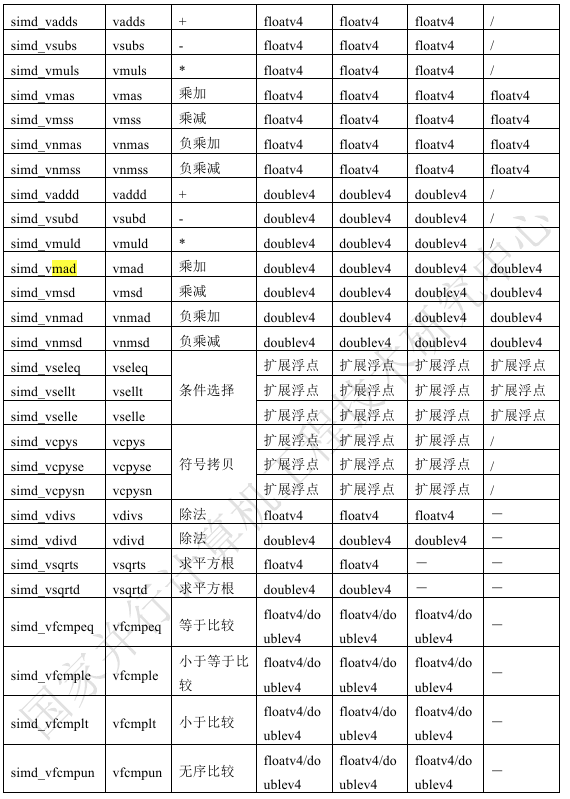
\includegraphics[width=12cm]{figure/sunway-simd.png}
  \end{center}

\subsubsection{Source code}
 We have compiled and executed the following source codes:

\verb`param.h`
\begin{code}
#define N 4096
#define I 64
#define Iv4 16

\end{code}

\verb`master.c`
\begin{code}
#include <stdlib.h>
#include <stdio.h>
#include <athread.h>
#include <sys/types.h>
#include <sys/stat.h>
#include <fcntl.h>

#include "param.h"

extern SLAVE_FUN(func)();

double a[N];
double b[N];
double c[N];

int main() {
  int i;
  printf("hello Sunway TaihuLight\n");

  for (i=0; i<N;++i){
    a[i] = i;
    b[i] = i;
  }

  // for (i=0; i<N;++i){
  //   c[i] = a[i] * b[i];
  // }
  athread_init();
  athread_spawn(func,0);//fflush(NULL);
  athread_join();

  for (i=1; i<N; i=2*i+1){
    printf("%d^2 == %lf\n", i, c[i]);
  }
  athread_halt();
  return 0;
}

\end{code}

\verb`slave.c`
\begin{code}
#include <slave.h>
#include <math.h>
#include <dma.h>

#include "param.h"

__thread_local volatile unsigned long get_reply, put_reply;
__thread_local doublev4 a_slave[Iv4], b_slave[Iv4], c_slave[Iv4];
extern double a[N], b[N], c[N];

void func() {
  int i;
  int my_id = athread_get_id(-1);
  int cid = my_id%8, rid = my_id/8;

  get_reply = 0;

  athread_get(PE_MODE, &a[my_id*I], &a_slave[0],I*8,&get_reply,0,0,0);
  athread_get(PE_MODE, &b[my_id*I], &b_slave[0],I*8,&get_reply,0,0,0);
  while(get_reply!=2) {}

  for(i=0;i<Iv4;i++){
    c_slave[i]=a_slave[i]*b_slave[i];
  }

  put_reply=0;
  athread_put(PE_MODE,&c_slave[0],&c[my_id * I],I*8,&put_reply,0,0);
  while(put_reply!=1) {}

}

\end{code}

\verb`run.sh`
\begin{code}

cd /home/export/base/nsccwuxi_riken/riken/online1/sandbox/nushio_box/sunway-test/03-slave-vector/src/
make && make run
    
\end{code}

\subsubsection{Results}

Got the following results:

\begin{code}
# 2017-02-14 13:05:28.457861
$ chmod 755 /home/nushio/hub/GB17/sunway-test/03-slave-vector/src/run.sh
$ ssh sunway 'mkdir -p /home/export/base/nsccwuxi_riken/riken/online1/sandbox/nushio_box/sunway-test/03-slave-vector/src/'
$ rsync -avz /home/nushio/hub/GB17/sunway-test/03-slave-vector/src/ sunway:/home/export/base/nsccwuxi_riken/riken/online1/sandbox/nushio_box/sunway-test/03-slave-vector/src/
sending incremental file list
./
Makefile
master.c
param.h
run.sh
slave.c

sent 1,385 bytes  received 117 bytes  429.14 bytes/sec
total size is 2,064  speedup is 1.37
$ ssh sunway /home/export/base/nsccwuxi_riken/riken/online1/sandbox/nushio_box/sunway-test/03-slave-vector/src//run.sh
sw5cc.new -O3 -msimd -host -E master.c > master.e
#	sw5cc.new -O3 -msimd -host -s master.c -o master.s
sw5cc.new -O3 -msimd -host -c master.c -o master.o
sw5cc.new -O3 -msimd -slave -E slave.c > slave.e
#sw5cc.new -O3 -msimd -slave -s slave.c -o slave.s
sw5cc.new -O3 -msimd -slave -c slave.c -o slave.o
sw5cc.new -hybrid  master.o slave.o -o main.out
bsub -I -b -q q_sw_expr -n 1 -cgsp 64 -share_size 4096 -host_stack 128 ./main.out
Job <6418407> has been submitted to queue <q_sw_expr>
some node is sleeping, waiting for dispatch ...
hello Sunway TaihuLight
1^2 == 1.000000
3^2 == 9.000000
7^2 == 49.000000
15^2 == 225.000000
31^2 == 961.000000
63^2 == 3969.000000
127^2 == 16129.000000
255^2 == 65025.000000
511^2 == 261121.000000
1023^2 == 1046529.000000
2047^2 == 4190209.000000
4095^2 == 16769025.000000
dispatching ...
Job 6418407 has been finished.

\end{code}

\subsubsection{Discussion}


We heve rewritten the previous example using
SIMD types and SIMD operations.


\subsection{Communicating between CPEs}
\subsubsection{Introduction}

CPEs form an 8x8 array, and
we can send the data in the row or the column direction in the CPE array.

The intrinsic functions
\verb`simd_putr` and
\verb`simd_putc` are used to send the data in the row nad the column direction, while
\verb`simd_getr` and
\verb`simd_getc` are used to recieve the data.

The second argument to the
\verb`simd_putr` and
\verb`simd_putc` functions
is the destination address. The address can be one of
(0...7) which specifies a column/row. The address can also be 8,
which means a broadcast.



\subsubsection{Source code}
 We have compiled and executed the following source codes:

\verb`param.h`
\begin{code}
#define N 256
#define I 4
#define Iv4 1

\end{code}

\verb`master.c`
\begin{code}
#include <stdlib.h>
#include <stdio.h>
#include <athread.h>
#include <sys/types.h>
#include <sys/stat.h>
#include <fcntl.h>

#include "param.h"

extern SLAVE_FUN(move_r)();
extern SLAVE_FUN(move_c)();

double a[N];
double b[N];
double c[N];

int main() {
  int i;
  athread_init();

  for (i=0; i<N;++i){
    a[i] = i/4;
    b[i] = i/4;
  }

  printf("before:");
  for (i=0; i<N; i++){
    if(i%4==0) printf(" ");
    if(i%32==0) printf("\n");
    printf("%2.0lf", a[i]);
  }
  printf("\n");

  athread_spawn(move_r,0);
  athread_join();

  printf("after move_r:");
  for (i=0; i<N; i++){
    if(i%4==0) printf(" ");
    if(i%32==0) printf("\n");
    printf("%2.0lf", c[i]);
  }
  printf("\n");

  athread_spawn(move_c,0);
  athread_join();

  printf("after move_c:");
  for (i=0; i<N; i++){
    if(i%4==0) printf(" ");
    if(i%32==0) printf("\n");
    printf("%2.0lf", c[i]);
  }
  printf("\n");

  athread_halt();
  return 0;
}

\end{code}

\verb`slave.c`
\begin{code}
#include <slave.h>
#include <math.h>
#include <dma.h>

#include "param.h"

__thread_local volatile unsigned long get_reply, put_reply;
__thread_local doublev4 a_slave[Iv4], b_slave[Iv4], c_slave[Iv4];
extern double a[N], b[N], c[N];

void move_r() {
  int i;
  int my_id = athread_get_id(-1);
  int cid = my_id%8, rid = my_id/8;

  get_reply = 0;

  athread_get(PE_MODE, &a[my_id*I], &a_slave[0],I*8,&get_reply,0,0,0);
  athread_get(PE_MODE, &b[my_id*I], &b_slave[0],I*8,&get_reply,0,0,0);
  while(get_reply!=2) {}

  simd_putr(a_slave[0], (cid+1)%8);
  c_slave[0] = simd_getr(c_slave[0]);

  put_reply=0;
  athread_put(PE_MODE,&c_slave[0],&c[my_id * I],I*8,&put_reply,0,0);
  while(put_reply!=1) {}

}

void move_c() {
  int i;
  int my_id = athread_get_id(-1);
  int cid = my_id%8, rid = my_id/8;

  get_reply = 0;

  athread_get(PE_MODE, &a[my_id*I], &a_slave[0],I*8,&get_reply,0,0,0);
  athread_get(PE_MODE, &b[my_id*I], &b_slave[0],I*8,&get_reply,0,0,0);
  while(get_reply!=2) {}

  simd_putc(b_slave[0], (rid*3)%8);
  c_slave[0] = simd_getc(c_slave[0]);

  put_reply=0;
  athread_put(PE_MODE,&c_slave[0],&c[my_id * I],I*8,&put_reply,0,0);
  while(put_reply!=1) {}

}

\end{code}

\verb`run.sh`
\begin{code}

cd /home/export/base/nsccwuxi_riken/riken/online1/sandbox/nushio_box/sunway-test/04-slave-comm/src/
make && make run
    
\end{code}

\subsubsection{Results}

Got the following results:

\begin{code}
# 2017-02-15 00:36:05.867609
$ chmod 755 /home/nushio/hub/GB17/sunway-test/04-slave-comm/src/run.sh
$ ssh sunway 'mkdir -p /home/export/base/nsccwuxi_riken/riken/online1/sandbox/nushio_box/sunway-test/04-slave-comm/src/'
$ rsync -avz /home/nushio/hub/GB17/sunway-test/04-slave-comm/src/ sunway:/home/export/base/nsccwuxi_riken/riken/online1/sandbox/nushio_box/sunway-test/04-slave-comm/src/
sending incremental file list
./
master.c
run.sh

sent 532 bytes  received 78 bytes  135.56 bytes/sec
total size is 2,906  speedup is 4.76
$ ssh sunway /home/export/base/nsccwuxi_riken/riken/online1/sandbox/nushio_box/sunway-test/04-slave-comm/src//run.sh
sw5cc.new -O3 -msimd -host -E master.c > master.e
#	sw5cc.new -O3 -msimd -host -s master.c -o master.s
sw5cc.new -O3 -msimd -host -c master.c -o master.o
sw5cc.new -hybrid  master.o slave.o -o main.out
bsub -I -b -q q_sw_expr -n 1 -cgsp 64 -share_size 4096 -host_stack 128 ./main.out
Job <6419585> has been submitted to queue <q_sw_expr>
waiting for dispatch ...
before: 
 0 0 0 0  1 1 1 1  2 2 2 2  3 3 3 3  4 4 4 4  5 5 5 5  6 6 6 6  7 7 7 7 
 8 8 8 8  9 9 9 9 10101010 11111111 12121212 13131313 14141414 15151515 
16161616 17171717 18181818 19191919 20202020 21212121 22222222 23232323 
24242424 25252525 26262626 27272727 28282828 29292929 30303030 31313131 
32323232 33333333 34343434 35353535 36363636 37373737 38383838 39393939 
40404040 41414141 42424242 43434343 44444444 45454545 46464646 47474747 
48484848 49494949 50505050 51515151 52525252 53535353 54545454 55555555 
56565656 57575757 58585858 59595959 60606060 61616161 62626262 63636363
after move_r: 
 7 7 7 7  0 0 0 0  1 1 1 1  2 2 2 2  3 3 3 3  4 4 4 4  5 5 5 5  6 6 6 6 
15151515  8 8 8 8  9 9 9 9 10101010 11111111 12121212 13131313 14141414 
23232323 16161616 17171717 18181818 19191919 20202020 21212121 22222222 
31313131 24242424 25252525 26262626 27272727 28282828 29292929 30303030 
39393939 32323232 33333333 34343434 35353535 36363636 37373737 38383838 
47474747 40404040 41414141 42424242 43434343 44444444 45454545 46464646 
55555555 48484848 49494949 50505050 51515151 52525252 53535353 54545454 
63636363 56565656 57575757 58585858 59595959 60606060 61616161 62626262
after move_c: 
 0 0 0 0  1 1 1 1  2 2 2 2  3 3 3 3  4 4 4 4  5 5 5 5  6 6 6 6  7 7 7 7 
24242424 25252525 26262626 27272727 28282828 29292929 30303030 31313131 
48484848 49494949 50505050 51515151 52525252 53535353 54545454 55555555 
 8 8 8 8  9 9 9 9 10101010 11111111 12121212 13131313 14141414 15151515 
32323232 33333333 34343434 35353535 36363636 37373737 38383838 39393939 
56565656 57575757 58585858 59595959 60606060 61616161 62626262 63636363 
16161616 17171717 18181818 19191919 20202020 21212121 22222222 23232323 
40404040 41414141 42424242 43434343 44444444 45454545 46464646 47474747
dispatching ...
Job 6419585 has been finished.

\end{code}

\subsubsection{Discussion}

We have confirmed that
\verb`simd_putr` sends the data in the row direction, and
\verb`simd_putc` sends the data in the column direction.


\subsection{SIMD arithmetic instructions (TODO)}
\subsubsection{Introduction}

We need to use the SIMD intrinsics of Sunway TaihuLight to make use of its full computing potential.
The SIMD intrinsic expressions accept SIMD types such as
\verb`intv8`,
\verb`doublev4`,
\verb`floatv4`.


We will test the effects of the SIMD intrinsics.


\subsubsection{Source code}
 We have compiled and executed the following source codes:

\verb`param.h`
\begin{code}
#define N 4096
#define I 64
#define Iv4 16

\end{code}

\verb`master.c`
\begin{code}
#include <stdlib.h>
#include <stdio.h>
#include <athread.h>
#include <sys/types.h>
#include <sys/stat.h>
#include <fcntl.h>

#include "param.h"

extern SLAVE_FUN(func)();

double a[N];
double b[N];
double c[N];

int main() {
  int i;
  printf("hello Sunway TaihuLight\n");

  for (i=0; i<N;++i){
    a[i] = i;
    b[i] = i;
  }

  // for (i=0; i<N;++i){
  //   c[i] = a[i] * b[i];
  // }
  athread_init();
  athread_spawn(func,0);//fflush(NULL);
  athread_join();

  for (i=1; i<N; i=2*i+1){
    printf("%d^2 == %lf\n", i, c[i]);
  }
  athread_halt();
  return 0;
}

\end{code}

\verb`slave.c`
\begin{code}
#include <slave.h>
#include <math.h>
#include <dma.h>

#include "param.h"

__thread_local volatile unsigned long get_reply, put_reply;
__thread_local doublev4 a_slave[Iv4], b_slave[Iv4], c_slave[Iv4];
extern double a[N], b[N], c[N];

void func() {
  int i;
  int my_id = athread_get_id(-1);
  int cid = my_id%8, rid = my_id/8;

  get_reply = 0;

  athread_get(PE_MODE, &a[my_id*I], &a_slave[0],I*8,&get_reply,0,0,0);
  athread_get(PE_MODE, &b[my_id*I], &b_slave[0],I*8,&get_reply,0,0,0);
  while(get_reply!=2) {}

  for(i=0;i<Iv4;i++){
    c_slave[i]=a_slave[i]*b_slave[i];
  }

  put_reply=0;
  athread_put(PE_MODE,&c_slave[0],&c[my_id * I],I*8,&put_reply,0,0);
  while(put_reply!=1) {}

}

\end{code}

\verb`run.sh`
\begin{code}

cd /home/export/base/nsccwuxi_riken/riken/online1/sandbox/nushio_box/sunway-test/05-slave-sqrt/src/
make && make run
    
\end{code}

\subsubsection{Results}

Got the following results:

\begin{code}
# 2017-02-15 13:46:19.548559
$ chmod 755 /home/nushio/hub/FDPS/sandbox/nushio_box/sunway-test/05-slave-sqrt/src/run.sh
$ ssh sunway 'mkdir -p /home/export/base/nsccwuxi_riken/riken/online1/sandbox/nushio_box/sunway-test/05-slave-sqrt/src/'
$ rsync -avz /home/nushio/hub/FDPS/sandbox/nushio_box/sunway-test/05-slave-sqrt/src/ sunway:/home/export/base/nsccwuxi_riken/riken/online1/sandbox/nushio_box/sunway-test/05-slave-sqrt/src/
sending incremental file list
run.sh

sent 173 bytes  received 40 bytes  28.40 bytes/sec
total size is 2,062  speedup is 9.68
$ ssh sunway /home/export/base/nsccwuxi_riken/riken/online1/sandbox/nushio_box/sunway-test/05-slave-sqrt/src//run.sh
sw5cc.new -O3 -msimd -host -E master.c > master.e
#	sw5cc.new -O3 -msimd -host -s master.c -o master.s
sw5cc.new -O3 -msimd -host -c master.c -o master.o
sw5cc.new -O3 -msimd -slave -E slave.c > slave.e
#sw5cc.new -O3 -msimd -slave -s slave.c -o slave.s
sw5cc.new -O3 -msimd -slave -c slave.c -o slave.o
sw5cc.new -hybrid  master.o slave.o -o main.out
bsub -I -b -q q_sw_expr -n 1 -cgsp 64 -share_size 4096 -host_stack 128 ./main.out
Job <6420164> has been submitted to queue <q_sw_expr>
waiting for dispatch ...
hello Sunway TaihuLight
1^2 == 1.000000
3^2 == 9.000000
7^2 == 49.000000
15^2 == 225.000000
31^2 == 961.000000
63^2 == 3969.000000
127^2 == 16129.000000
255^2 == 65025.000000
511^2 == 261121.000000
1023^2 == 1046529.000000
2047^2 == 4190209.000000
4095^2 == 16769025.000000
dispatching ...
Job 6420164 has been finished.

\end{code}

\subsubsection{Discussion}

TODO


\subsection{Using the C++ compiler}
\subsubsection{Introduction}

You can use C++ compiler in TaihuLight.



\subsubsection{Source code}
 We have compiled and executed the following source codes:

\verb`master.cpp`
\begin{code}
#include <stdlib.h>
#include <stdio.h>
#include <athread.h>
#include <sys/types.h>
#include <sys/stat.h>
#include <fcntl.h>

#define N 4096


extern SLAVE_FUN(func)();

double a[N];
double b[N];
double c[N];

int main() {
  int i;
  printf("hello Sunway TaihuLight\n");

  for (i=0; i<N;++i){
    a[i] = i;
    b[i] = i;
  }

  // for (i=0; i<N;++i){
  //   c[i] = a[i] * b[i];
  // }
  athread_init();
  athread_spawn(func,0);//fflush(NULL);
  athread_join();

  for (i=1; i<N; i=2*i+1){
    printf("%d^2 == %lf\n", i, c[i]);
  }
  athread_halt();
  return 0;
}

\end{code}

\verb`slave.c`
\begin{code}
#include <slave.h>
#include <math.h>
#include <dma.h>

#define N 4096
#define I 64

__thread_local volatile unsigned long get_reply, put_reply;
__thread_local int my_id;
__thread_local double a_slave[I], b_slave[I], c_slave[I];
extern double a[N], b[N], c[N];

void func() {
  int i;
  my_id = athread_get_id(-1);
  get_reply = 0;

  athread_get(PE_MODE, &a[my_id*I], &a_slave[0],I*8,&get_reply,0,0,0);
  athread_get(PE_MODE, &b[my_id*I], &b_slave[0],I*8,&get_reply,0,0,0);
  while(get_reply!=2) {}

  for(i=0;i<I;i++){
    c_slave[i]=a_slave[i]*b_slave[i];
  }

  put_reply=0;
  athread_put(PE_MODE,&c_slave[0],&c[my_id * I],I*8,&put_reply,0,0);
  while(put_reply!=1) {}

}

\end{code}

\verb`run.sh`
\begin{code}

cd /home/export/base/nsccwuxi_riken/riken/online1/sandbox/nushio_box/sunway-test/02-slave/src/
make && make run
    
\end{code}

\subsubsection{Results}

Got the following results:

\begin{code}
TODO

\end{code}

\subsubsection{Discussion}

TODO


